\RequirePackage{fix-cm}
\documentclass[anonymous,12pt]{iopjournal}
\usepackage{amsmath,amssymb,amsthm,booktabs,array,graphicx,placeins}
\graphicspath{{figures/}}
\hypersetup{hidelinks,pdftitle={Material-set inversion with fixed constitutive traces and conditional scattering operators},pdfauthor={}}
\fancyhead[L]{\small\sffamily Inverse Problems\quad Research paper}
\fancyhead[R]{\small Material-set inversion}
\setlength{\headheight}{17pt}
\setlength{\emergencystretch}{2em}
\renewcommand{\topfraction}{.94}
\renewcommand{\bottomfraction}{.9}
\renewcommand{\textfraction}{.06}
\newtheorem{theorem}{Theorem}[section]
\newtheorem{proposition}[theorem]{Proposition}
\newtheorem{corollary}[theorem]{Corollary}
\newcommand{\C}{\mathbb C}
\newcommand{\R}{\mathbb R}
\newcommand{\Bd}{\mathcal B}
\newcommand{\A}{\mathcal A}
\newcommand{\Po}{P_{\mathrm o}}
\newcommand{\ReH}{\operatorname{Re}_{H}}
\newcommand{\ImH}{\operatorname{Im}_{H}}
\newcommand{\diag}{\operatorname{diag}}
\newcommand{\ran}{\operatorname{ran}}
\newcommand{\tr}{\operatorname{tr}}
\newcommand{\np}{n_+}
\newcommand{\nn}{n_-}
\newcommand{\Tail}{\mathcal T}
\numberwithin{equation}{section}
\begin{document}
\noindent{\sffamily\small RESEARCH PAPER}\par\vspace{1.8ex}
\title{Material-set inversion with fixed constitutive traces and conditional scattering operators}
\author{}
\begin{abstract}
Finite-aperture scattering data can rule out an entire dielectric inclusion class, although they may leave individual pixels undetermined. We derive two results for the discrete nonlinear transverse magnetic volume integral equation. First, a family of material intervals that changes on a fixed set of cells admits a common exact reduction. Retaining the current and total-field traces there recovers the inertia of every data test up to a known positive block, including singular cases. Second, when the old readings exhaust the available negative directions, every compatible material satisfies a conditional quadratic bound on its response to future illumination. A separate index computed from the old sources determines whether this bound is an ellipsoid. In 24 material pairs the full and reduced tests agreed on all 2688 material hypotheses. Imposing exact laws on selected unknown cells gave no additional exclusions beyond exact elimination of known vacuum. On a 9216-cell model the data ruled out 247 of 256 positions for a core of specified size, with one verified compatible position and eight unresolved. In six finite-aperture examples a single additional beam separated two previously compatible classes. A uniform angle also achieved this result. The conditional bound establishes when a future beam suffices before its response is measured. On the native array a physically compatible class leaves seven receiving directions uncontrolled at saturation even with 32 illuminations. For a narrower class, eleven coherent beams above a calculated energy threshold yield a bounded receiving prediction; eleven angular beams at the same energy leave five directions uncontrolled.
\end{abstract}

\par\smallskip
\keywords{inverse medium scattering, material uncertainty, finite aperture, set inversion, illumination design}
\section{Introduction}
A microwave array measures exterior fields. In a material calibration experiment the quantity of interest may be the contrast of an inclusion in a specified region, or the position of a high-contrast core. Both questions survive a change in the surrounding material. To rule out a proposed core position, every allowed distribution in its surrounding layer and background must miss the measured fields. Conversely, one distribution fitting the data at that position establishes its physical possibility. The two conclusions require different calculations. We study both for a finite, noisy array with multiple scattering retained.

The relevant structure connects two uses of the same apparatus. On changing a dielectric hypothesis at a cell, only the relation between its induced current and total field changes. The Green function and receiver remain fixed. On changing the illumination of a fixed dielectric, the full scattering response is linear in the incident field, even when its dependence on material is strongly nonlinear. We use the first fact to compare entire material classes and the second to ask which future readings a surviving class could produce. A future illumination can then be selected by a statement about all materials still under consideration.

Subspace inversion methods separate currents visible to the receiver from an ambiguous component \cite{chen,zhong,ffttsom}. They use the integral equation and the common contrast to recover an image. Local conservation bounds constrain electromagnetic responses \cite{kuang,moleskylocal,trivedi}, and cross-field identities enforce common structure in multifunctional design \cite{shim}. Here a receiver residual and its error radius enter the same form as the local material constraints. An indefinite state block is allowed. This is essential when a few reactive current directions can offset material constraints without explaining all incident fields simultaneously.

Several mathematical precedents delimit this approach. Port reduction and static condensation eliminate internal variables in parametrized component problems \cite{huynh}. We retain selected cell fields and currents, together with the nonpositive directions of a common state block. The reduction preserves the full inertia at every noise threshold for the stated family. Interval set inversion supplies the logic of outer covering and retention \cite{sivia}. Monotonicity in inverse medium and obstacle scattering compares probe regions against a far-field operator up to finite-dimensional exceptions \cite{griesmaier_harrach,griesmaier_harrach_erratum,albicker}. Our exception count belongs to an interior current form at the measured finite ports. It does not require a continuum far-field operator.

In interpolation theory a bounded number of negative squares restricts extensions of a Pick matrix \cite{pick}. In guaranteed active diagnosis an input can be chosen so that bounded output sets for different models become disjoint \cite{scott}. The contribution here is to obtain such output sets from a common dielectric law, old complex readings and a fixed full-wave Green operator. We identify a source-side obstruction that can be tested before a particular realization of the old readings is known. This distinguishes a failure of the chosen physical bound from a failure of a particular new illumination. Our numerical tests separate exclusion, physical compatibility and unresolved classes. The results concern the specified discrete model, with a separate accounting of errors when measured fields are used.
\section{What the measurements imply about a material interval}\label{sec:material}
\subsection{Physical model and data distance}
We use time dependence $\exp(-{\rm i}\omega t)$ and an out-of-plane electric field in a nonmagnetic, two-dimensional dielectric. If $k$ is the host wavenumber and $\chi$ the relative permittivity contrast, the polarization current in our normalization is $j=\chi e$. Factors of $k^2$ are included in the Green operator. The outgoing kernel for distinct points is $\mathrm{i}k^2 H_0^{(1)}(k|x-x'|)/4$ \cite{colton,richmond}. For pulse cells the field is collocated at cell centres. In the equal-area disk rule a cell of equivalent radius $a$ has self coefficient $\mathrm{i}\pi ka H_1^{(1)}(ka)/2-1$. Specific quadrature and port normalization are part of each discrete model.

Let $G\in\C^{n\times n}$ map currents to internal scattered fields, $S\in\C^{p\times n}$ map currents to the receivers, and $\Bd\in\C^{n\times m}$ contain fields of available physical illuminations. Columns of $V\in\C^{m\times s}$ specify the transmitted beams and $B=\Bd V$. With $X=\diag(\chi_i)$,
\begin{equation}
 E=B+GJ,\qquad J=XE,\qquad Y_{\rm clean}=SJ .
 \label{eq:physics}
\end{equation}
Receiver whitening acts on both $S$ and $Y$. A box $\ell_i\leq\chi_i\leq u_i$ specifies the allowed real material independently in every free cell. In vacuum $j_i=0$ exactly. Physical well-posedness gives the response $\mathcal F_X=S(I-XG)^{-1}X\Bd$ to the dictionary. The basic rejection test also applies to all field solutions when the forward equation is interpreted as a relation. Predicting a response to a new beam requires a common linear response to all beams.

For measured $Y$ and joint Frobenius error radius $r$, we bound the infimum of $\|SJ-Y\|_F$ over the class and its physical states. A strict lower endpoint above $r$ excludes the class. A particular material in the class with a verified upper residual at most $r$ establishes compatibility. If neither conclusion follows, the class stays in the cover.

\subsection{The material law as a quadratic form}
Write $Z=[V^\top,Y^\top]^\top$. The two quantities on which the local material acts are the current row $j_i$ and the field row $e_i$ across all illuminations. With $q_i$ the coordinate vector for cell $i$, set
\begin{equation}
 z_i=\begin{bmatrix}j_i\\e_i\end{bmatrix}=T_iJ+E_iZ,\quad
 T_i=\begin{bmatrix}q_i^\top\\q_i^\top G\end{bmatrix},\quad
 E_i=\begin{bmatrix}0&0\\q_i^\top\Bd&0\end{bmatrix}.
 \label{eq:trace}
\end{equation}
At every real material row $j_i=\chi_i e_i$ the optical cross product $\ImH(j_i^*e_i)$ vanishes, where $\ImH A=(A-A^*)/(2{\rm i})$.
Let $m_i=(u_i+\ell_i)/2$, $h_i=(u_i-\ell_i)/2$, $w_i\geq0$, $\lambda_i\in\R$. Then
\begin{align}
 D_i&=\begin{bmatrix}w_i&-w_i m_i-{\rm i}\lambda_i/2\\
                     -w_i m_i+{\rm i}\lambda_i/2&w_i\ell_i u_i\end{bmatrix},\notag\\
 z_i^*D_i z_i&=w_i(\chi_i-\ell_i)(\chi_i-u_i)e_i^*e_i\preceq0 .
 \label{eq:sector}
\end{align}
Off-diagonal entries of the $s$ by $s$ source Gram matrix couple different beams through the same real material. Adding \eqref{eq:sector} to the squared data residual gives
\begin{equation}
 \A=[S,0,-I_p]^*[S,0,-I_p]+\sum_i[T_i,E_i]^*D_i[T_i,E_i]
   =\begin{bmatrix}K&-R_0\\-R_0^*&D_0\end{bmatrix}.
 \label{eq:form}
\end{equation}
For physical currents $D_{\rm res}=(SJ-Y)^*(SJ-Y)\succeq[J;Z]^*\A[J;Z]$. A semicolon inside brackets denotes vertical concatenation. All terms are formed in the original current coordinates. The state block, linear term and constant term can all change when the material bounds change.

\begin{proposition}[Testing the distance]\label{prop:count}
Set $\A_Z=\diag(I_n,Z)^*\A\diag(I_n,Z)$ and $P_s=\diag(0_n,I_s)$. If $1\leq j\leq s$, $t\geq0$, $jt\geq r^2$ and $\np(\A_Z-tP_s)\geq n+j$, the full class misses the noise ball. If $K$ is nonsingular, set $\nu=\nn(K)$ and $H=Z^*(D_0-R_0^*K^{-1}R_0)Z$. A lower bound on the squared distance is
\begin{equation}
 \Tail_\nu(H)=\sum_{i=\nu+1}^{s}\max\{\lambda_i^\downarrow(H),0\}.
 \label{eq:tail}
\end{equation}
\end{proposition}
\begin{proof}
The graph $[J;I_s]$ has dimension $s$. It intersects a positive subspace of $\A_Z-tP_s$ in at least $j$ dimensions. Compression to source space gives at least $j$ eigenvalues of $D_{\rm res}$ strictly above $t$. For invertible $K$, completing the square gives $D_{\rm res}\succeq H+U_+^*U_+-U_-^*U_-$, with at most $\nu$ negative rows. The inertia additivity and interlacing used here are classical \cite{haynsworth,tian,fan}. Interlacing the rank-$\nu$ subtraction and using $D_{\rm res}\succeq0$ gives \eqref{eq:tail}.
\end{proof}
An exact uncoupled null state may be divided out and $n$ reduced by its dimension. A zero state coupled to the source must remain. Small numerical eigenvalues alone give no permission to remove a direction.

\begin{proposition}[Sharpness of the rank information]\label{prop:sharp}
Under only $D\succeq0$, $D\succeq H-U^*U$ and $U\in\C^{\nu\times s}$, the minimum of $\tr D$ equals $\Tail_\nu(H)$.
\end{proposition}
\begin{proof}
For fixed $U$, the positive spectral projector of $H-U^*U$ gives a trace lower bound attained by $D=(H-U^*U)_+$. Interlacing gives \eqref{eq:tail}. Choose $U^*U$ equal to the largest $\min(\nu,\np(H))$ positive spectral components of $H$. Equality follows.
\end{proof}
An improved distance at fixed $K$ requires more information about realizable material or current. For one incident field the current derivatives at a regular interior point are the columns of $(I-XG)^{-1}\diag(e)$. When every component of $e$ is nonzero their complex linear span is $\C^n$. A fixed complex linear current space containing every current in the neighbourhood must have dimension $n$, even with a single receiver.

\subsection{A fixed reduction for a family of material classes}
Suppose the endpoints or multipliers vary only on a common set $R$. Stack the corresponding row pairs to obtain $T_R,E_R$. For a reference form $\A_b$,
\begin{equation}
 \A_\theta=\A_b+[T_R,E_R]^*D_\theta[T_R,E_R],
 \label{eq:update}
\end{equation}
where $D_\theta$ contains differences of the local blocks. The exterior may remain unknown throughout the family. A large unknown exterior and a large set of \emph{changes} to the reference form are distinct sources of computational cost.

\begin{theorem}[Exact fixed-trace reduction]\label{th:fixed}
Let the columns of $U$ be an orthonormal basis for $\ran T_R^*+\mathcal E_{\leq0}(K_b)$, of dimension $d$. Let $W$ span the orthogonal complement orthonormally. Then $C_+=W^*K_bW\succ0$ on that complement. In coordinates $[W,U,\mathrm{ports}]$ eliminate $C_+$ once from $\A_b$, obtaining $\widehat\A_b$. Set $F=[T_R U,E_R]$ and $\widehat\A_\theta=\widehat\A_b+F^*D_\theta F$. For all $\theta,Z,t$, the full and reduced threshold forms have identical negative and zero indices. The full positive index exceeds the reduced index by $n-d$. There is no invertibility requirement on $K_b$, $K_\theta$ or $D_\theta$.
\end{theorem}
\begin{proof}
$W$ lies in the positive spectral space of $K_b$, and $T_R W=0$. Neither the eliminated block nor its couplings to the remaining variables changes in \eqref{eq:update}. A triangular congruence completes the square in its coordinates, leaving $C_+$ and the stated reduced block. Port substitution and the threshold act only on retained coordinates and commute with elimination. Sylvester's law gives the three counts.
\end{proof}

The dimension satisfies $d\leq\min\{n,2|R|+\dim\mathcal E_{\leq0}(K_b)\}$. Keeping actual receiver traces adds at most $\operatorname{rank} S$ rows. In computation an exact nullspace of selected trace covectors and a verified positive restriction suffice. Extra numerical covectors can define exactly specified additional coordinates. The test on their complement establishes positivity without identifying an approximate eigenbasis with an exact invariant subspace.

Nested intervals transfer information. Write $s_{\ell,u}(j,e)=(j-me)^*(j-me)-h^2e^*e$. For a parent and child with positive half-widths $h\geq h'$ and centres $m,m'$, $\lvert m'-m\rvert\leq h-h'$ implies
$(h/h')s_{\ell',u'}-s_{\ell,u}\succeq0$ on all row pairs. The difference of the two local forms has first diagonal entry $h/h'-1$ and determinant $(h/h')[(h-h')^2-(m-m')^2]\geq0$, with equality of the forms when $h=h'$. Multiplying the child sector weight by $h/h'$ preserves the parent test. A zero-width interval is an exact row and can inherit the parent's logical exclusion directly.

\subsection{Adding shared material rows}
Condensation alone cannot change a conclusion at fixed weights. A stronger constraint imposes $j_i=\xi_i e_i$ on chosen cells with one real $\xi_i\in[\ell_i,u_i]$ for every beam. After completing the positive square of $K_b$ write $J=J_c+P v+N c+N_0 d_0$, where $PP^*=K_{b,+}^{\dagger}$, $J_c=K_{b,+}^{\dagger}R_{0,b} Z$, and $c,d_0$ span the negative and null directions. For required traces $z$, put $\Sigma=TPP^*T^*$ and $b=z-EZ-T(J_c+Nc+N_0d_0)$. A positive-space completion exists exactly when $\ran b\subseteq\ran\Sigma$. Its smallest matrix energy is
\begin{equation}
 \min_{TPv=b}v^*v=b^*\Sigma^\dagger b .
 \label{eq:completion}
\end{equation}
The minimizer is $(TP)^\dagger b$. Every other completion adds a vector orthogonal to its range, proving the assertion in Loewner order. Retaining the receiver trace makes this an equivalence for the mixed model with the aggregate quadratic constraint and the selected exact rows. Further exact rows give nested outer material sets. Equivalence to \eqref{eq:physics} requires all material rows, including any known background row not eliminated exactly.

For an additional predicted row pair $(\widehat j_i,\widehat e_i)$ let $\Sigma_{i|R}$ be its conditional trace Gram after the preceding rows. With $a_\xi=(1,-\xi)$, the additional minimum energy is
\begin{equation}
 \frac{(\widehat j_i-\xi\widehat e_i)^*(\widehat j_i-\xi\widehat e_i)}
 {a_\xi\Sigma_{i|R}a_\xi^*}.
 \label{eq:innovation}
\end{equation}
This follows by imposing the single linear innovation after \eqref{eq:completion}. At a zero denominator the numerator must vanish. A trace score in a fixed source direction is a ratio of real quadratics, so endpoints and stationary points suffice for ranking. A ranking evaluated on a trial state cannot by itself exclude a material. Verification enforces the chosen equations jointly over their full intervals.

For this calculation one adds their traces to \eqref{eq:update}, drops their now redundant sector terms, and solves a verified nonsingular pivot of the shared row equations. The retained state takes the form $x=N_\xi v+X_\xi Z$ throughout a subinterval. Substitution leaves the source threshold unchanged. A positive frame valid throughout the subinterval proves the same count on the reduced number of free states. Failed pivots and inconclusive frames prompt subdivision. A parent is removed only when all its leaves are removed. The procedure requires no numerical cutoff on the free negative coordinates. Uniform strict margins and a regular chart cover give finite termination by compactness. The number of subdivisions can grow exponentially with the number of shared variables.

\section{What a surviving class can scatter next}\label{sec:response}
\subsection{An operator determined by the old readings}
Let $K$ be nonsingular. Eliminating current at stationary energy in \eqref{eq:form} gives a fixed port form
\begin{equation}
 Q=D_0-R_0^*K^{-1}R_0,\qquad H=Z^*QZ,\qquad \Po=H-\Omega .
 \label{eq:Q}
\end{equation}
Here $\Omega\succeq D_{\rm old}$ is valid for every compatible medium. With a joint Frobenius error ball one can take $\Omega=r^2 I_s$. The errors may be coherent across beams: two equal unit errors have Gram matrix with largest eigenvalue two. Separate unit column radii therefore do not justify $\Omega=I_2$. If only separate bounds $r_i$ are known, one possible common upper matrix is $(\sum_i r_i^2)I_s$.

\begin{theorem}[Conditional scattering operator]\label{th:response}
Assume each compatible material admits a common linear clean response on the dictionary. Let $\nu=\nn(K)$ and suppose $\Po$ is nonsingular with $\np(\Po)=\nu$. Define
\begin{equation}
 Q_c=Q-QZ\Po^{-1}Z^*Q
   =\begin{bmatrix}Q_{aa}&Q_{ay}\\Q_{ya}&R_y\end{bmatrix}.
 \label{eq:qc}
\end{equation}
Every compatible material satisfies $[I;\mathcal F_X]^* Q_c[I;\mathcal F_X]\preceq0$.
If $R_y\succ0$, let $C_a=-R_y^{-1}Q_{ya}$ and $\Theta=Q_{ay}R_y^{-1}Q_{ya}-Q_{aa}$. Then
\begin{equation}
 (\mathcal F_X-C_a)^*R_y(\mathcal F_X-C_a)\preceq\Theta .
 \label{eq:ellipse}
\end{equation}
A nonempty class implies $\Theta\succeq0$.
\end{theorem}
\begin{proof}
Consider any set of clean future responses $Z_\star=[A_\star;\mathcal F_X A_\star]$ for the same material. Their residuals vanish identically, including their cross terms with old errors. The augmented residual Gram is bounded above by $\diag(\Omega,0)$. The rank bound in proposition~\ref{prop:count} then gives
\begin{equation}
 \np\begin{bmatrix}\Po&Z^*Q Z_\star\\Z_\star^*QZ&Z_\star^*QZ_\star\end{bmatrix}\leq\nu .
 \label{eq:aug}
\end{equation}
The old block already has $\nu$ positive directions. Its Schur complement is nonpositive. Taking $A_\star=I_m$ and completing the receiving square proves both assertions.
\end{proof}
Old measurement uncertainty has already entered $\Po$. Only the error on the future acquisition dilates the clean response set. If $\Po$ has a known exact nullspace with basis $U_o$, saturation also forces $U_o^*Z^*QZ_\star=0$. A nonzero coupling to this kernel creates an extra positive direction. After imposing this condition, $\Po^\dagger$ replaces $\Po^{-1}$ in \eqref{eq:qc}. At an unresolved near-zero eigenvalue we retain the bordered condition. If $K$ itself has a proven nullspace $N_0$, the port form is a descriptor pair: eliminate the invertible part and retain the zero block with coupling $-N_0^*R_0 Z$. Substituting $K^\dagger$ in \eqref{eq:Q} alone would lose that coupling.

When $k_o=\np(\Po)<\nu$, appending $m_\star$ rows and columns increases the positive index by at most $m_\star$. For $m_\star\leq\nu-k_o$, \eqref{eq:aug} holds for every hypothetical reading. At least $\nu-k_o+1$ further columns are therefore needed for this particular index test to distinguish anything. The necessity concerns a fixed form and error majorant. A different material restriction, multiplier or joint trace bound may give information sooner.

\subsection{A source-side test for bounded prediction}\label{sec:sourceindex}
Saturation does not by itself bound the next receiver field. The receiving block in \eqref{eq:qc} must also be positive. There is a way of testing this second requirement without constructing responses for trial receivers. Remove the measured power term from \eqref{eq:form} and write its material part on currents and old illuminations as
\begin{align}
 \mathcal P_o&=
 \begin{bmatrix}K_{\rm mat}&-N V\\-V^*N^*&V^*C_{\mathcal B}V-\Omega\end{bmatrix},
\notag\\
 K_{\rm mat}&=K-S^*S,\qquad R_0=[N,S^*],\qquad D_0=\diag(C_{\mathcal B},I_p).
 \label{eq:sourceform}
\end{align}
The early absence of receiver directions is an algebraic consequence of allowing the whole receiver field to vary.

\begin{proposition}[Receiver index from the material and the old sources]\label{prop:sourceindex}
For invertible $K,\Po$, put $h_{\rm src}=n-\np(\mathcal P_o)$. Then
\begin{equation}
 \np(R_y)=p-h_{\rm src}+\nu-\np(\Po).
 \label{eq:index}
\end{equation}
If there is at least one material in the class with a physical solution for the old illuminations then $h_{\rm src}\geq0$. At saturation, bounded prediction by the positive receiving square is possible precisely when $h_{\rm src}=0$. In particular $s<\nn(K_{\rm mat})$ rules it out even at saturation.
\end{proposition}
\begin{proof}
Take the form on a current $x$, old source coefficients $v$ and a freely varying receiver vector $y$. Its value is the material form on $(x,Vv)$ plus $\|Sx-Yv-y\|^2-v^*\Omega v$. Translating $y$ yields a direct sum of $I_p$ and $\mathcal P_o$. Eliminating $x$ and then $v$ instead yields $K,\Po,R_y$. Equality of positive indices and $\np(K)=n-\nu$ prove \eqref{eq:index}. The graph of any common material solution has dimension $s$ and is nonpositive for $\mathcal P_o$. Thus $\np(\mathcal P_o)\leq n$. Finally, bordering $K_{\rm mat}$ by $s$ columns can add at most $s$ positive directions.
\end{proof}
For fixed $\Omega,V$, material intervals and weights, $h_{\rm src}$ is independent of the values of $Y$ and of the particular receiving array. The array and the measurement still determine whether saturation occurs and the size and position of a bounded set. The proposition permits an inexpensive rejection of unsuitable weights if only a lower bound $\nn(K_{\rm mat})>s$ is known. For invertible $K_{\rm mat}$ a small source form gives the exact deficit,
\begin{equation}
 h_{\rm src}=\nn(K_{\rm mat})
 -\np\!\left(V^*(C_{\mathcal B}-N^*K_{\rm mat}^{-1}N)V-\Omega\right).
 \label{eq:indexsmall}
\end{equation}
At a singular material block \eqref{eq:sourceform} still applies directly. Rank deficiency of the original dielectric inverse map is a different property.

\subsection{Incident energy needed for a bounded receiver set}
The source test has a useful design consequence when coherent mixtures of the dictionary are available. Assume $K_{\rm mat}$ invertible, set $q=\nn(K_{\rm mat})$, $Q_s=C_{\mathcal B}-N^*K_{\rm mat}^{-1}N$ and let the incident-energy Gram $W_{\rm in}$ be positive definite on the allowed dictionary. Energy is $\tr(V^*W_{\rm in}V)$. We keep the old error majorant $\Omega=\sigma^2 I_s$, $\sigma>0$, fixed while choosing $V$. Write $\beta_1\ge\cdots\ge\beta_m$ for the eigenvalues of $W_{\rm in}^{-1/2}Q_sW_{\rm in}^{-1/2}$.

\begin{corollary}[Energy needed to remove the source deficit]\label{cor:energy}
Suppose that one material in the class has a physical solution on the full incident dictionary and $q>0$. If $m<q$, $s<q$, or the available $q$th eigenvalue satisfies $\beta_q\le0$, no energy budget removes $h_{\rm src}$. Otherwise the infimum of the energy needed for $h_{\rm src}=0$ is
\begin{equation}
 E_{\rm inf}=\sigma^2\sum_{i=1}^{q}\beta_i^{-1}.
 \label{eq:energy}
\end{equation}
Every budget strictly greater than this infimum suffices. At $q=0$ the source deficit is always zero.
\end{corollary}
\begin{proof}
Applying the material graph argument with $V=I$ and zero error gives $\np(Q_s)\le q$. By \eqref{eq:indexsmall}, zero deficit requires a $q$-dimensional beam subspace on which $V^*Q_sV\succ\sigma^2 I$. Restrict to orthonormal source coordinates on that subspace and write the whitened restricted synthesis matrix as $UT$, with $U^*U=I_q$ and $T$ invertible. Put $A=U^*W_{\rm in}^{-1/2}Q_sW_{\rm in}^{-1/2}U$. Then $T^*AT\succ\sigma^2 I$ implies $TT^*\succ\sigma^2 A^{-1}$. The energy exceeds $\sigma^2\tr A^{-1}\ge E_{\rm inf}$ by eigenvalue interlacing. Choosing the leading generalized eigenbeams with energies just above $\sigma^2/\beta_i$ attains the infimum in the limit.
\end{proof}
This is a requirement for the fixed quadratic prediction to bound every receiving direction at saturation. It does not guarantee saturation, separation of two material classes, or a particular material reconstruction. A finite menu of physical angles can require more energy. An exposure-dependent error model requires a new calculation.


\subsection{Selecting an illumination before observing its response}
A source vector $a$ with incident energy $a^*W_{\rm in}a$ produces a clean field in an ellipsoid centred at $C_a a$. In receive direction $w$, its real support radius is
\[
 b(a,w)=\sqrt{a^*\Theta a}\sqrt{w^*R_y^{-1}w}.
\]
For classes $i,j$ and one future noise radius $r_a$, the separation margin for a chosen $(a,w)$ is
\begin{equation}
 \operatorname{Re}w^*(C_j-C_i)a-b_i(a,w)-b_j(a,w)-2r_a\|w\| .
 \label{eq:gap}
\end{equation}
A verified positive margin implies at most one of these two material classes can explain the new reading. The decision is made before that reading exists. With $\|w\|\leq1$, maximizing the clean gap gives exactly the Euclidean distance between the two closed convex ellipsoids (zero if they intersect). Weak duality follows from the support functions. For disjoint compact sets the direction from one closest point to the other attains the distance. This is a receiver-space second-order cone problem \cite{boyd}. A verified trial direction suffices for exclusion even when it is suboptimal.

For a batch $A_\star$, \eqref{eq:ellipse} gives clean fields in
$C_iA_\star+R_i^{-1/2}\Delta(A_\star^*\Theta_iA_\star)^{1/2}$, $\|\Delta\|_2\leq1$. The matrix support radius for test $W$ is
$\|R_i^{-1/2}W(A_\star^*\Theta_iA_\star)^{1/2}\|_*$ by spectral/nuclear norm duality. This keeps cross-beam correlations. A Frobenius bound $r_\star$ adds $r_\star\|W\|_F$ to each end. For independent deterministic column bounds $r_j$, the sharper exact support is $\sum_j r_j\|W_{:,j}\|_2$. Beams in the span of the old incident fields have no independent clean response; repeating a beam may have statistical value under a separate noise model.

A single regular form has a restriction here. At saturation with $R_y\succ0$, $\Theta$ is positive semidefinite for any box that contains a material regular on the entire dictionary, even if that material fails to fit the old readings. Indeed, free the source $a$ and the receiver $y$ in the form on $(x,v,a,y)$ with port data $(Vv+a,Yv+y)$ and old penalty $v^*\Omega v$. Eliminating $x,v,y$ gives $K\oplus\Po\oplus R_y\oplus(-\Theta)$. Translating $a,y$ instead gives the material form on $(x,a)$, $-\Omega$ and $I_p$. The material solution graph has dimension $m$ and is nonpositive, so the latter sum has at most $n+p$ positive directions. The former has $n+p+\nn(\Theta)$, proving the claim. This argument requires the stated nonsingular pivots.

There is also an old-data consistency test. If two valid forms for the \emph{same} class yield disjoint clean receiving projections for a common hypothetical illumination, that class is already empty. Otherwise a single physical material would have to scatter that beam into both projections. No new beam need be fired for this implication. In a three-cell algebraic control two individually nonrejecting tail bounds gave disjoint intervals with gap greater than 0.05542. An ordinary uniform weight also rejected this example. Five further physical material boxes that the original test could not exclude also survived this paired-form test. The control verifies the implication without establishing an advantage over weight search.

For more than two classes, connect pairs with a proven positive margin. Each clique contributes at most one survivor. Any clique cover gives a worst-case survivor bound, even if a greedy cover is used. This counts only the classes in the specified cover. To attain the displayed bound after acquisition, compare the new reading with the stored old-data support intervals enlarged by its new error first. Then append the new columns and run the joint material test. A single joint Frobenius bound can discard the separate error information used by the support test.

\section{Which spatial questions admit a map?}\label{sec:space}
\subsection{A cover of core centres}
A physically high value in one cell and an inclusion with a finite core are different observations about a material. For a region $D$, the assertion $\max_{i\in D}\chi_i\ge t$ is a union over cells. Excluding one cell from this union establishes that a peak cannot lie in that cell. To conclude $\max_{i\in D}\chi_i<t$ one must exclude every member. Conversely, excluding the single box $\chi_i\le t$ throughout $D$ establishes that a peak above $t$ exists somewhere in $D$. It does not locate the peak. A specified shape with uncertain amplitude defines a third query, with a separate interval at every cell of the prescribed profile.

Consider a class with unknown centre $c$, an inner set $I_c$ guaranteed to have contrast at least $u$, an outer set $O_c$ within which contrast can reach $U$, and background $[0,b]$ elsewhere, $0\le b<u\le U$. No proportionality is required between neighbouring cells. The annular and paired-inclusion versions use translated annular and paired templates. For a square of centre labels $C$ form
\begin{equation}
 I_C=\bigcap_{c\in C} I_c,\qquad O_C=\bigcup_{c\in C} O_c .
 \label{eq:map}
\end{equation}
The single box with mandatory core $I_C$, allowed outer region $O_C$ and background cap $b$ contains every material attached to every $c\in C$. This follows directly by testing each coordinate against the least lower endpoint and largest upper endpoint. Excluding this box excludes the whole square of centres. Otherwise subdivide the centre labels or keep every label at the current resolution. A witness is assigned only to centres for which its material satisfies the bounds. An unresolved centre denotes an outer possibility. This remains true when a parent has empty common core.

The number of centre labels is two-dimensional even though the individual material values inside the boxes are independent. For the single fixed subspace of theorem~\ref{th:fixed}, its dimension depends on the union of cells that change between tests. When the common state block is positive definite, a moving-support implementation can instead store and query the trace Gram of a larger library. It can be large near the root of the tree. Subdivision at such a node preserves coverage without running a costly test there. For a discrete centre grid the coverage stops at the stated labels. Continuous centres require conservative coverage of the variation within each centre tile as well.

\subsection{Loss of a bound and loss of information}
In a fixed material test, enlarging the outer background from $[0,b_0]$ to $[0,b_0+\delta]$ changes the original sector form affinely. In the notation of proposition~\ref{prop:count}, write the threshold matrix as $A_0-\delta T_O$. If a positive test frame $Q_+$ gives $G_0=Q_+^*A_0Q_+\succ0$, it stays positive precisely while
\begin{equation}
 I-\delta\,G_0^{-1/2}Q_+^*T_OQ_+G_0^{-1/2}\succ0 .
 \label{eq:toler}
\end{equation}
A positive largest eigenvalue gives a limiting expansion equal to its reciprocal. A nonpositive largest eigenvalue permits arbitrary positive expansion of this frame, subject to the declared model. We hold the weights, basis and noise event fixed here. The calculation measures the range of one proof. It cannot establish that two different materials produce the same fields.

There is a separate physical mechanism for indistinguishability. Let $f(\theta,z)$ be the independent real and imaginary measurements after removing exact redundancies. Here $\theta$ describes a task and $z$ the unknown background. At a regular interior material the derivative in a real material direction $d$ is the real representation of
\begin{equation}
 S(I-XG)^{-1}\diag(d)(I-GX)^{-1}B .
 \label{eq:deriv}
\end{equation}
If $A_b=D_zf$ has full row rank, choose a right inverse $R_b$ and set $z=z_0+R_b v$. The implicit function theorem applied to $f(\theta,z_0+R_bv)-f(\theta_0,z_0)$ produces a background adjustment that preserves the complete nonlinear data for sufficiently small task changes. Interior slack keeps it legal. Quantitatively, if $\phi(v)=f(\theta,z_0+R_bv)-f(\theta_0,z_0)$ satisfies $\|D_v\phi-I\|\le\eta<1$, and the initial defect is at most $a$, mapping a ball of radius $a/(1-\eta)$ into itself gives a background cost at most $\|R_b\|_{2\to\infty}a/(1-\eta)$. An interval proof must verify the derivative bound, the domain of that ball and the material slack. When $A_b$ lacks full row rank, projection orthogonal to its range detects an uncompensated first-order effect; vanishing of this projection alone gives no nonlinear ambiguity.

A three-cell example illustrates the size of the adjustment. At one complex reading, shifting the task contrast from 0.70 to 0.74 can be offset by moving the two background values from $(0.0625,0.0625)$ to approximately $(0.03723,0.08443)$. The background derivative has full real rank two. For the stored discrete operator a real resultant has a sign-changing rational bracket, and a uniform resolvent bound keeps the denominator nonzero. Thus equality of the complex reading in this example is exact.

An isolated peak illustrates the remaining limitation. Around $X_0$ define $T_0=(I-GX_0)^{-1}G$, $P_0=S(I-X_0G)^{-1}$ and $E_0=(I-GX_0)^{-1}B$. Increasing cell $i$ by $d$ produces exactly
\begin{equation}
 \Delta Y=\frac{d}{1-d(T_0)_{ii}}\,
          (P_0 q_i)(q_i^\top E_0).
 \label{eq:spike}
\end{equation}
The single-cell total-field equation gives the denominator and the exterior propagation supplies the two field factors. For a regular update the signal can fall below a prescribed noise radius despite large $d$. For example, with bounded fields and denominator bounded away from zero, refining a distant cell reduces its radiating area. A minimum core size specifies precisely the additional physical information used in \eqref{eq:map}.

\section{Material classes, core positions and future measurements}\label{sec:experiments}
We use the same three outcomes throughout. An \emph{excluded} hypothesis has a one-sided distance bound above the specified radius. A \emph{witness} is an actual material whose original field equations give a residual upper endpoint inside the ball. Anything else is \emph{unresolved}. Exclusion applies to the entire tested class. A witness proves existence. It can occur in several overlapping classes. Statistics below count independent materials separately from repeated measurements, widths and proof operations. All source choices use only the specified material prior and measurements already made.

\subsection{Amplitude and geometry under uncertain background}
A set of 24 independently generated pairs gives 48 base materials. Each is measured on four paired background realizations. Sixteen pairs share precisely the same nonzero cells and differ in amplitude. Eight share the same allowed region with different internal structures. To test both directions of the inverse question each material in a pair supplies data in turn and both candidate classes are tested. We determined the geometry families, parameter bands, noise and methods before generating the hidden materials. Sealed decisions precede comparisons with the generating arrays.

The controlled comparison uses 25 independent real cells on a square of side $0.70$ wavelengths, eight plane waves, twelve receiving directions over a half aperture and a $1.5\%$ joint complex noise level. Eight cells define the changing task region. Outside it the material is either known vacuum or free in $[0,b]$, with $b=1/32,1/16,1/8$. The background realization is paired between the two members of each amplitude pair. We use seven box half-widths, $0.5,0.9,1,1.5,2,3,5$ times a centre-dependent Neumann scale. The scale is the reciprocal of the reference feedback norm on the active cells in vacuum. Clipping enforces the material domain. The abscissa specifies the design; actual divergence is checked separately.

\begin{table}[tb]\centering
\caption{Decisions on 2688 data--class tests from 24 independent pairs. Cost is seconds summed over the common set. Search includes shared assembly when a method uses it. The second pair of cost columns distinguishes producing and independently checking a bound. Shared physical witness search and checking cost a further 21.7 s.}\label{tab:a}
\small
\begin{tabular}{@{}lrrrrrr@{}}\toprule
 & Excluded & Witness & Unresolved & Search & Bound & Replay\\\midrule
Directional perturbation &244&1488&956&1.65&59.50&3.70\\
Positive state form &925&1488&275&57.17&105.00&81.04\\
Indefinite state form &1116&1488&84&37.28&12.16&15.35\\
Fixed traces &1116&1488&84&26.87&3.61&12.56\\
Additional shared rows &1124&1488&76&2.30$^a$&38.21$^a$&0.08$^a$\\\bottomrule
\end{tabular}
\par\smallskip\parbox{.93\linewidth}{\footnotesize $^a$Increment over fixed traces. The reduced form also uses 6.50 s for the common base solves and about 0.20 s for the realisation of the multiplier bank. The same search limits and physical boxes apply to all five rows.}
\end{table}
The perturbation comparison uses \eqref{eq:neumann} with directional support of the linear term and an outward remainder. The positive-state comparison combines spatially independent multipliers and multiple source directions with separately chosen positive-state quadratic bounds. Positivity and the resulting sum of directional bounds are checked in the original coordinates. These are finite searches over specified multipliers and source frames. The numbers in table~\ref{tab:a} do not assert an optimum over all positive semidefinite dual representations. The full and reduced indefinite calculations use the same multiplier bank. The final row permits one, two, four or eight exact local material rows on cases that remain unresolved. A matched positive-state check used the complete positive source eigenspace, hence $\tr(H_+)$, for all 72 common weights at which $K\succ0$ could be verified. Across all 2688 tests it gave 1026 exclusions, 1488 witnesses and 174 unresolved. The search, proof and independent replay cost 34.16, 14.84 and 12.05 s in addition to the reference comparison. For the remaining 90 exclusions, all 6480 state matrices were checked. Of these 6446 had a strictly negative direction. For each of the remaining 34 positive states the positive-tail upper bound was below the noise threshold (maximum squared bound divided by squared radius 0.96439). The difference therefore holds throughout this finite weight bank.

All 1464 tests whose literal box contains the generating material retained it, including all 1344 generating paths. All 192 original measurements also admitted the generating material under independent full-wave checking, with residual upper endpoint below $0.999934r$. Of 1224 opposite-class boxes that did not contain that particular material, 32 had a different full-wave witness. For one same-profile pair at background cap $1/8$ and relative width three, data from a material of peak 3.87949 also admit a peak of 3.83695. The latter has residual at most 0.056287 against a radius of 0.060268. The active task-cell support agrees; the two legal backgrounds can differ. A procedure counting every opposite-class label as erroneous would misreport these genuine ambiguities. At the same weights the full and reduced forms agreed on every one of the 2688 decisions. Of their 1116 exclusions, 408 used a state block verified to be indefinite. In 119 distinct material boxes (192 data--box tests) an allowed perturbation had spectral radius greater than one.

\begin{figure}[tb]\centering
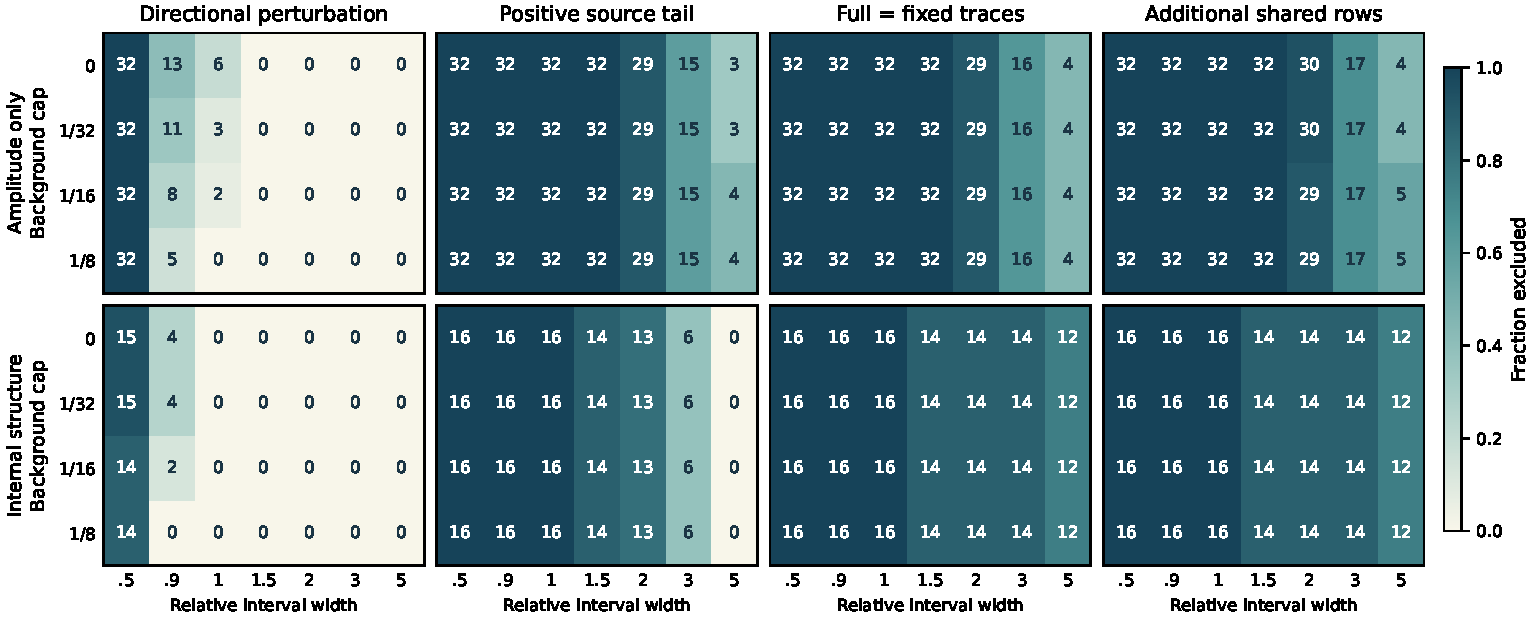
\includegraphics[width=.96\linewidth]{phase_comparison}
\caption{Exclusion over relative interval width and the allowed background. Each panel uses the stated physical hypothesis and shows the fraction of the opposite boxes outside the generating material which could be excluded. Methods and denominators refer to identical measurements in each comparison. Numbers are counts excluded. Positive-state comparisons include the full positive source tail. Full and fixed-trace tests agreed in every cell. Blank entries have no eligible boxes.}\label{fig:phase}
\end{figure}
Figure~\ref{fig:phase} distinguishes amplitude tests at identical support from changes of internal structure. A mechanism check explains the apparent gain from local realization: the eight additional exclusions arose in three amplitude pairs, and every successful local equation had interval $[0,0]$. Of 633 attempts, 388 selected at least one row with positive width. None of those attempts supplied an additional exclusion. An independent calculation that first set all known vacuum currents to zero and then applied ordinary full inertia reproduced all eight and gave twenty more. It left 56 hypotheses unresolved. The sharpness proposition therefore guides the interpretation: additional material information can help, but the results here favour exact use of known vacuum before refinement in unknown cells. The scalar rows remain a valid increasing hierarchy. For a separate cold-start convex comparison after the same vacuum elimination, we took both readings and both classes of all eight structural pairs at relative width three. The positive semidefinite search and the indefinite calculation each gave 14 exclusions and 18 witnesses on all 32 tests. The respective search and checking times were 198.88 and 0.209 s plus 0.327 and 0.017 s for independent checking (including the initial indefinite check in the latter 0.017 s). This comparison concerns the cost of attaining the same answers.

We also considered two larger physical controls at 400 MHz on a two-metre square, using 32 transmitters and 32 receivers. The native model has $96^2$ cells. Precisely 1153 are allowed to carry nonzero material. The measured low disk (peak 0.625) occupies 416 cells, and the hollow ring (peak 3.50) occupies 768. The competing solid profile uses all 1153. Its material can vary independently across these cells. The two calculations share a permitted active region; their actual supports differ. With $2\%$ error, the data distances to the competing class exceeded $1.7284r$ and $3.5945r$, respectively. The class widths were 5.14 and 3.09 times their reference contraction scales. For explicit permitted perturbations $\rho(wT)>1.0864$ and $>1.3896$, respectively. The halo outside the stated active region is known vacuum. The relative first Born error of the hollow ring is $376\%$.

The size of the search region materially changes this comparison. Figure~\ref{fig:scaling} shows 28 independent $96^2$ media on a two-metre domain ($ka=11.85$) and seven compact $24^2$ media. For the former, at $10\%$ noise the full-aperture Born class and nonlinear peak cap 0.5 were excluded on all 28, whereas the chosen bounds excluded cap 0.75 on none. For the compact set the joint bound excluded cap five on five of seven and the material of peak 4.28 supplies a physically legal control. These are distinct data and material contracts. The compact comparison has $ka=4.27$, twelve incident fields, 48 receiving ports and $1\%$ noise; the large-domain comparison has ten fields and 20 ports. Here $a$ is the enclosing radius of the computational square. The numbers identify a limitation of unrestricted peak inference in one aperture and electrical size. They do not define a geometry-independent limiting contrast. The angular bandwidth of radiated fields is itself a scale, not a strict finite rank \cite{bucci87}.
\begin{figure}[tb]\centering
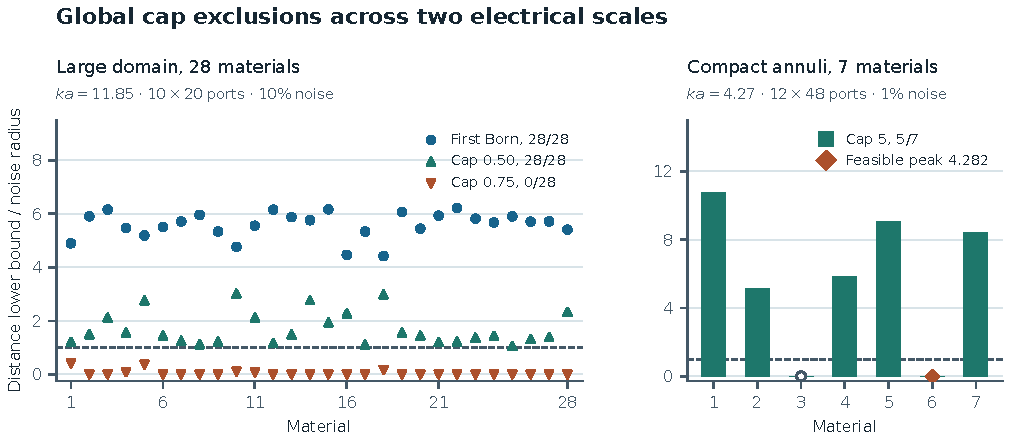
\includegraphics[width=.93\linewidth]{scaling}
\caption{Independent materials at two electrical sizes. A point above one excludes the stated hypothesis. A point at or below one measures the limit of the calculation. In the right panel one material is known to be within the proposed cap. Material indices are local to each panel.}\label{fig:scaling}
\end{figure}

\subsection{Mapping a core without an initial image}
We next tested the question a map answers. On a $12^2$ grid there were seven transmitted beams and nine receiving ports on arcs, at 135 MHz on a two-metre square. The noise radius was $3\%$, with a small allowance for forward arithmetic. We generated three independent objects, a disk, two inclusions and an annulus. Inside the mandatory core each cell could vary in $[0.75,1.375]$, in the outer layer in $[0,1.375]$, and in the background in $[0,b]$. The paired and annular templates preserve their stated separation and cavity. The unknowns included every permitted material value and the discrete centre in the pictured search window. The centre tree started from the whole window.

\begin{figure}[tb]\centering
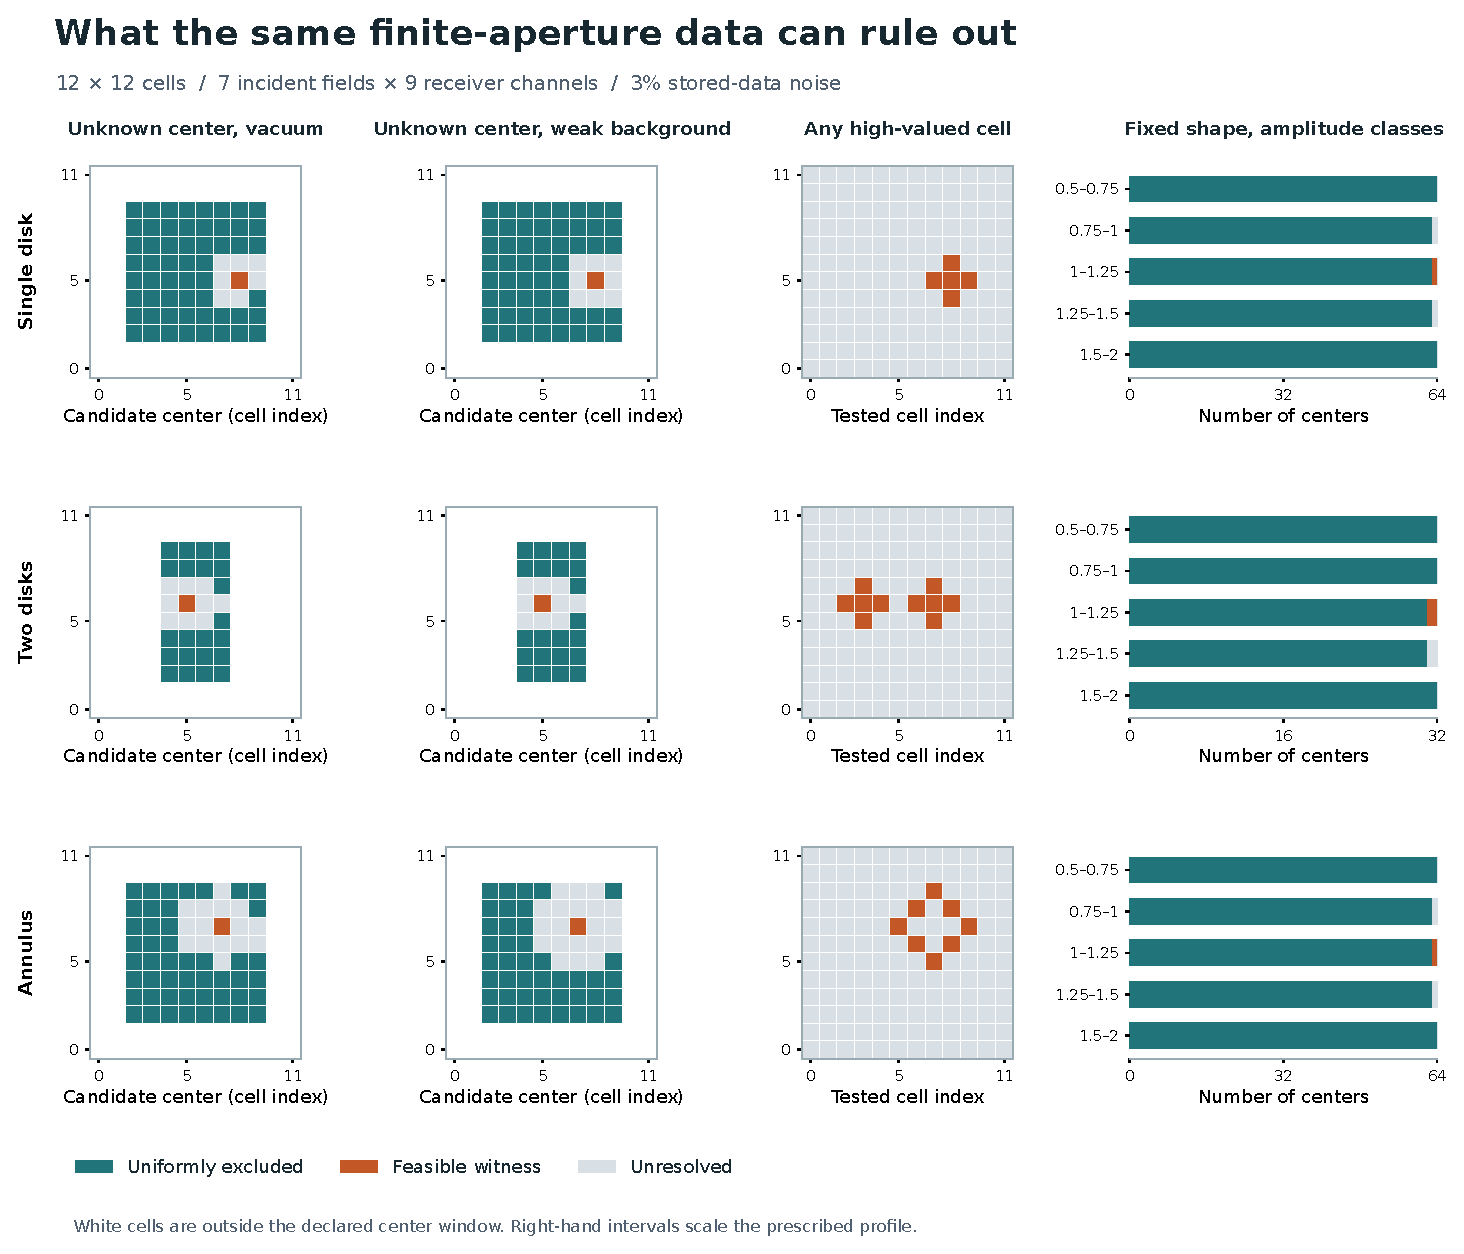
\includegraphics[width=.95\linewidth]{spatial-map}
\caption{Spatial hypotheses tested against the same complex readings. Centre maps ask where a specified finite core can occur; the single-cell query allows arbitrary material elsewhere. A compatible label requires an actual forward solution. Remaining labels may still be impossible.}\label{fig:map}
\end{figure}
With $b=1/32$, the numbers of excluded, compatible and unresolved centres were $(55,1,8)$ out of 64 for the disk, $(22,1,9)$ out of 32 for the two inclusions and $(43,1,20)$ out of 64 for the annulus. Setting $b=0$ raised the exclusion counts to 56, 22 and 48. Each material was also tested under a stated shape profile with five possible amplitude intervals. All three admitted a witness in $[1,1.25]$. The surviving interval hull was $[0.75,1.5]$ for the disk and ring and $[1,1.5]$ for the two inclusions. In contrast, on permitting all other cells to range freely in $[0,1.375]$, none of 432 propositions that a specified cell could reach one was ruled out. Twenty-three had witnesses (figure~\ref{fig:map}).

A separate $96^2$ experiment used seven transmitters and nine receivers drawn from the finite native arcs at 400 MHz, a $4\%$ error radius and a core of radius two cells, outer radius three and a vacuum exterior. On a $16$ by $16$ centre grid, 247 centres were excluded, one had an explicit witness with residual below $0.980r$, and eight remained unresolved. The computation descended through 21 parents whose allowed outer regions were too large for the chosen direct test. All 70 excluding nodes were checked against the original Fourier kernel. The result covers all 256 centres in this window even though many material coordinates were never subdivided.

\begin{figure}[tb]\centering
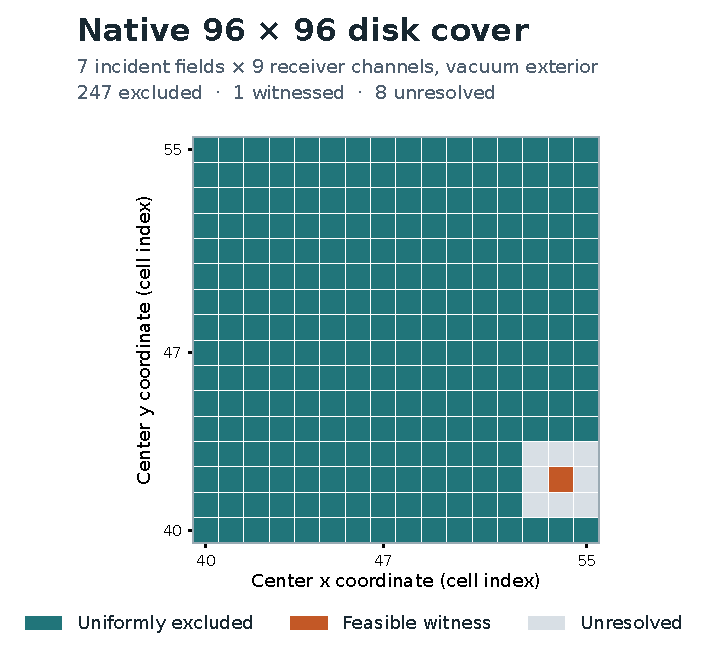
\includegraphics[width=.82\linewidth]{native-center-map}
\caption{Core position on the native grid. The seven transmitting angles run from $-67.5$ to $67.5$ degrees and the nine receiving angles from $-78.75$ to $67.5$ degrees. The result applies to an independently varying core and layer with the stated minimum thickness. The true material is used only for evaluation.}\label{fig:nativemap}
\end{figure}
A separate moving-support implementation used 100 and 1000 different boxes on 53 and 64 distinct nine-cell supports, respectively. The common state block was positive definite and each local update invertible. Precomputing the full trace Gram once allowed a small submatrix to be gathered for each support. A second bordered elimination with $-D_\theta^{-1}$ reduced the order from 151 to 25. These timings apply to this more restrictive moving-support algorithm; the fixed-row, singular-safe comparison of theorem~\ref{th:fixed} is the preceding 2688-box study. The machine-precision checks took 0.595 and 5.909 s in full coordinates, versus 0.018 and 0.154 s after reduction, with identical signs in every box. The reduced 128-bit computation for all boxes took 0.224 and 2.817 s after 0.598 and 0.736 s of cold preparation. Model construction, loading and box generation together took at most 0.046 s. Full-matrix interval rechecks of 16 and 32 boxes took 4.392 and 10.390 s. The strict decisions excluded 97 of 100 and 985 of 1000. These are distinct production and replay costs. The smaller floating-point times alone would overstate the end-to-end benefit.

\subsection{Can prospective illumination reduce the set?}
We tested the conditional operator on six independent synthetic media, two per geometry. All three arrays had three receivers. The first had unequal radii and asymmetric angles, the second used a $130$ degree arc, and the third kept three ports of a masked array. Masking a port did not insert a scattering obstacle. The square was $0.70$ wavelengths wide at 400 MHz, with a $4$ by $4$ discretization. For each object the task prior consisted of two competing interval material classes. Public nominal centres with near-equal old responses were prepared independently of the generating material, which was drawn within one class. Both nominal centres gave strictly compatible old full-wave fields in all 24 class--energy conditions in each of the following two comparisons.

We initially illuminated at $0$ and $180$ degrees. From ten further angles at $30$ degree spacing we selected batches of one, two or four, giving 10, 45 or 210 possible actions. In the added-energy regime each beam had unit incident fluence. In the fixed-total regime the two old beams were acquired separately at half energy each and one further unit was shared among the new beams. Noise was an absolute bound per receiving column. Each method had the same angular menu and the same post-acquisition tests. Random choice, uniform angular completion, a local nuisance-adjusted Fisher design and \eqref{eq:gap} were compared. Each proposal and its receiving direction were stored before calling the separate future-measurement program. After acquisition the stored support test was applied before repeating the joint inertia test.

At half-width $0.0008$ and absolute per-beam radius $0.00018$, all 3180 candidate actions across materials, energies and batch sizes had a strictly positive gap. Each policy removed the incorrect class on the first beam in all six media for both energy budgets. This establishes causality of the prospective calculation, but the menu was too easy to distinguish angular policies. We repeated the same media with four times the width and a radius of $2\%$ of the old added-energy RMS column norm. The rule was chosen before collecting the new readings for this comparison. It changes both width and noise, and adds no independent objects.

\begin{table}[tb]\centering
\caption{Number of the six media for which the selected batch provably separates the two classes before acquisition in the larger intervals. The last block gives wrong-class removals with the realized data. The three columns of each block correspond to one, two and four additional beams.}\label{tab:active}
\small\begin{tabular}{@{}lccc@{}}\toprule
Selection & Added fluence & Fixed total & Fixed total, realized\\\midrule
Random &5,5,6&3,3,3&6,5,6\\
Uniform angle &6,6,6&6,5,4&6,6,6\\
Nuisance-adjusted Fisher &6,6,6&5,5,3&6,6,6\\
Conditional response &6,6,6&6,6,4&6,6,6\\\bottomrule
\end{tabular}
\end{table}
In this comparison, 2016 of 3180 actions had a proven edge for the specified bounds. Only 345 of 1260 four-beam fixed-total actions did so. The four-beam menu had no proven edge for two of the six objects. Splitting a fixed energy among beams while keeping the absolute error per beam fixed can reduce guaranteed separation. The conditional choice increased the median one-beam support margin from 0.00765 for uniform completion to 0.01891. In both cases all six realized first beams sufficed. Of 144 realized paths, 143 removed the incorrect class; the saved support alone did so in all 143 and the joint update alone in 140. The remaining path was a random two-beam choice under fixed total energy. All 144 true material witnesses survived. These results concern the two stated priors, not all material images.

\begin{figure}[tb]\centering
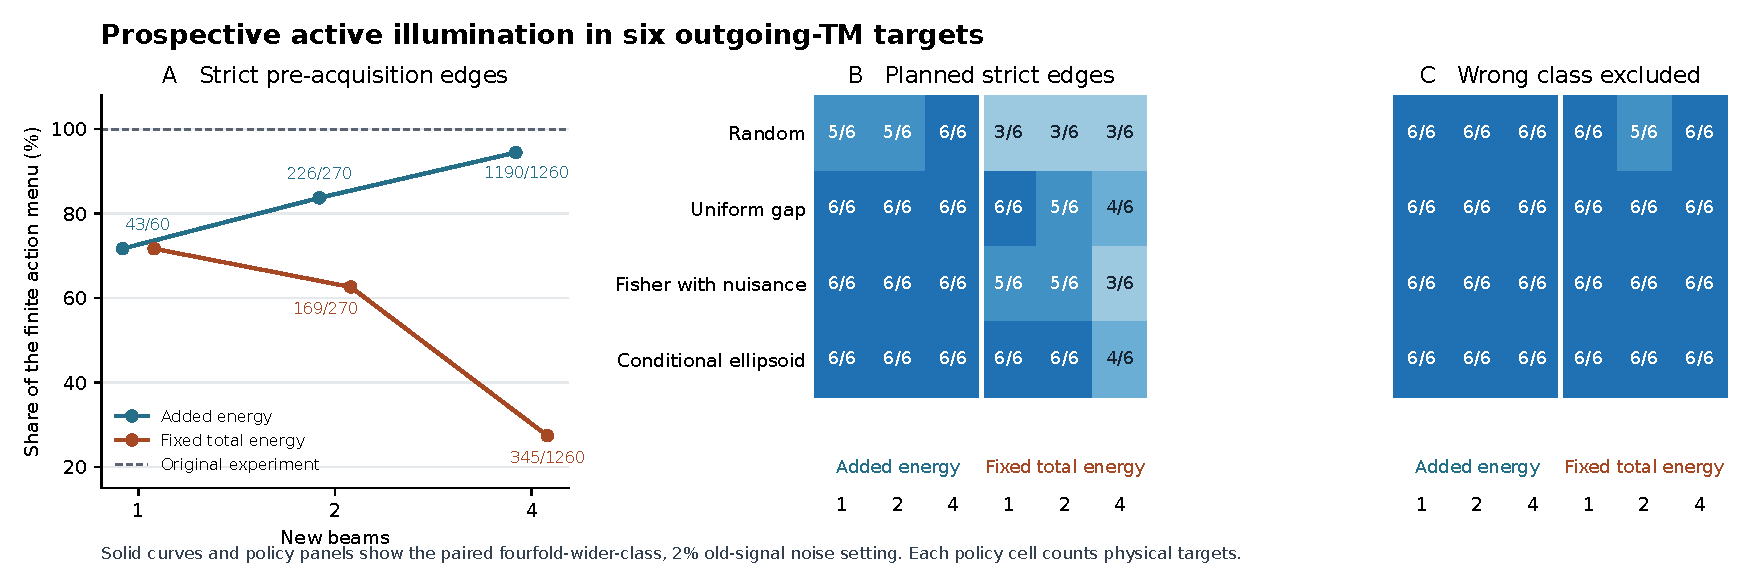
\includegraphics[width=.92\linewidth]{active_policy}
\caption{Prospective separation under different allocations of the same incident energy. Each line or cell summarizes the same six physical media. Success after observing a favourable reading can occur even when the old data provide no worst-case separation guarantee.}\label{fig:active}
\end{figure}
The positive-state weights on these narrow classes saturated and had a positive receiving block in all 192 weight tests in each comparison. All 96 broad indefinite trials on $[0,3]^{16}$ per comparison had an old index deficit. Thus the compact prospective demonstration uses positive-state weights. The frozen receive direction joined the predicted centres, with the joint Frobenius noise allowance applied to batches of columns. The four-beam shortfall is therefore specific to that direction, energy split and noise envelope. An old-data receiver-space cone optimization on all 120 single-beam choices of the sensitivity study improved each of the 86 positive margins, while the same 86 choices remained separated. The other 34 supplied no strict separation in either calculation.

A further test used the same two occupied classes of each compact object and the same old readings, with positive sector weights and a signed optical multiplier on one cell. Both class forms in all six objects had $\nu=k_o=1$ and a positive receiving square under the added-energy convention. For each of the 60 single-beam choices an interval-verified point on the line of their centres belonged to both clean response ellipsoids. No receive direction separates those two outer sets, even at zero future noise. The positive-state forms in the original experiment already separate the classes. This provides a full-wave indefinite example and isolates a genuine loss in the chosen outer bounds.

A separate native computation tests whether saturation and receiving positivity can fail independently. It uses the disk and hollow ring readings in the $1153$-cell active region, three fixed material forms, and prefixes of 1, 2, 4, 8, 16 and 32 old beams. The original full noise majorant is kept for every prefix as a conservative choice. Prediction from \eqref{eq:index} and direct interval inertia of the $32$ by $32$ receiving block agree on all 36 cases. In the solid class of half-width $2.5$, the disk data saturate with 16 and 32 beams ($k_o=\nu=13$), yet the receiving block has 25 positive and seven negative directions. At 32 beams the ring gives the same source-side deficit of seven, with $k_o=6$ and 32 positive receiving directions. Neither calculation gives the bounded conditional operator of theorem~\ref{th:response}. These prefix tests diagnose a fixed form; they do not establish old-data compatibility of a rival class.

A nonempty native example removes this last ambiguity. We acquired two synthetic beam readings from the centre of the solid class of half-width 1.5, keeping the same receiver, material form and error bound $r=0.0388901$. The resulting 64 complex values reproduce the complete two-beam forward solution to within $4.08\times10^{-17}$. Since $K\succ0$, the strict data slack makes $\Po\prec0$. Saturation here is automatic for compatible data at a positive definite state block. The material-only state has eleven negative directions, the old source pivot has two positive directions, and the receiving block has exactly 23 positive and nine negative directions. Here the shortage follows already from having two old beams for eleven material modes. This example establishes occupancy on the native grid. Its freely varying receiving square is indefinite even with arbitrarily accurate readings inside the stated error contract. Figure~\ref{fig:source} shows how this possibility arises.

\begin{figure}[tb]\centering
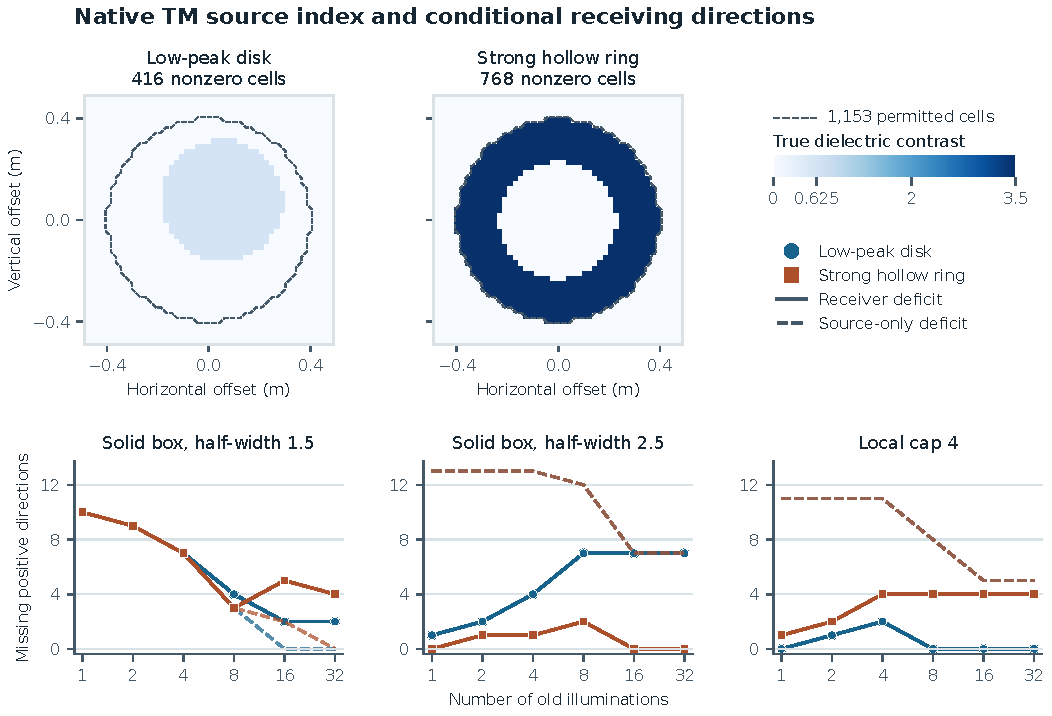
\includegraphics[width=.93\linewidth]{native-source-index}
\caption{Two measured materials within the same permitted region, and the two distinct index conditions. The dashed curves show the source-side deficit; solid markers show the number of missing positive receiver directions obtained by independent interval evaluation. The original noise radius for each object is used at every source count.}\label{fig:source}
\end{figure}
For the tighter solid interval, the 32 incident fields have eleven positive generalized source directions, exactly the number required by corollary~\ref{cor:energy}. In units of the incident intensity of one original beam summed over the full square, the infimum in \eqref{eq:energy} is in $[0.59082793,0.59082795]$ at the disk error radius and $[3.74429999,3.74430008]$ at the ring radius. The wider solid interval has thirteen negative material directions and only six positive dictionary directions. The corresponding uniform cap of four has eleven and six. Unlimited fluence in the same dictionary therefore leaves deficits of at least seven and five, respectively. This statement is independent of a particular old receiving record and is specific to its fixed spatial weight. No feed-network power calibration is assumed.

We tested this energy threshold with an occupied class (figure~\ref{fig:nativebeam}). Fix eleven exposures, the same per-column error allowance $r/\sqrt{11}$, and exactly $1.25 E_{\rm inf}$ incident fluence ($0.738535$ in these units). The plane-wave design takes eleven separated dictionary angles; the coherent design uses the leading generalized eigenbeams. Both see the same solid material, the same port geometry and the same normalized noise realization. Saturation holds for both. The coherent design makes $R_y$ positive definite ($\lambda_{\min}>0.00266$), while the angular design leaves five negative receiving directions. This is a strict difference in bounded prediction under one material form at equal incident energy.

The wider solid class was also tested with a physical material in its interior. With 16 and 32 ordinary beams, $\nu=k_o=13$ in both cases; direct evaluation gives 25 positive and seven negative receiving directions in both. This example has enough sources by count and a strictly compatible full-wave solution. Its deficit is the shortage of positive dictionary directions in \eqref{eq:indexsmall}. The narrower and wider tests shared one simultaneous 32-right-hand-side physical solve. Including validated spectral and receiving calculations, the narrow comparison took 78.75 s and the additional wide comparison 38.10 s.

\begin{figure}[tb]\centering
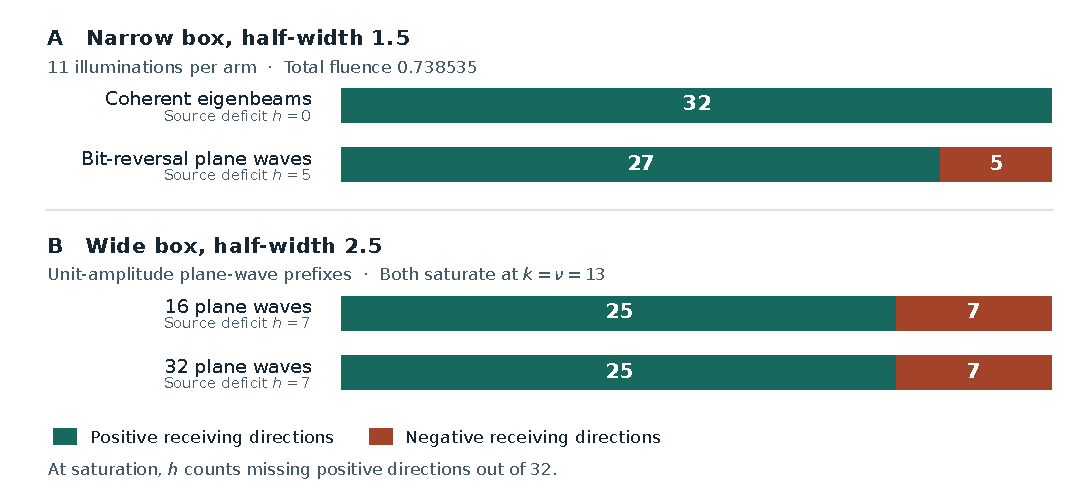
\includegraphics[width=.91\linewidth]{native-illumination}
\caption{Receiving directions on an occupied native material class. Left, identical fluence and eleven exposures per design. Right, nested ordinary-angle prefixes for the wider interval. In both panels a nonpositive receiving direction is a limit of the chosen bound on the scattered response.}\label{fig:nativebeam}
\end{figure}


\subsection{Model errors and microwave measurements}
Synthetic results above come with two distinct numerical error specifications. For the broad comparison the stored discrete matrices are the defined operator. For the compact prospective study the interval evaluation includes the equal-area disk and Hankel cell model itself. Both differ from a bound on replacing a physical continuum by that model. On one aligned square inclusion, evaluation of the discrete kernels on $8^2$ and $16^2$ grids enclosed the relative field difference between 0.04600043134948238 and 0.04600043134948240. On six other media compared on $96^2$ and $32^2$ at full and half aperture, individual differences ranged from $12.43\%$ to $35.43\%$. This is a sample discrepancy, not a uniform correction for all media in the class.

For a calibrated measurement $Y=(I+\Delta)F+\eta$ with $\|\Delta\|\le\epsilon<1$ and $\|\eta\|_F\le r_\eta$, the clean distance obeys
\begin{equation}
 \|F-Y\|_F\le(\epsilon\|Y\|_F+r_\eta)/(1-\epsilon).
 \label{eq:gain}
\end{equation}
Indeed $\|F-Y\|_F\le\epsilon(\|Y\|_F+\|F-Y\|_F)+r_\eta$. For common gain error $\mathrm i/32$ and additive error $1/2048$, interval arithmetic bounded the realized error by 0.016397 and the data-dependent upper bound by 0.017657.

We applied the error accounting to the Fresnel and Manitoba microwave data \cite{fresnel,manitoba}. There are seven physical specimens. The three Fresnel targets contribute nine target--frequency pairs at 4, 6 and 8 GHz. Four Manitoba targets contribute 28 pairs at 3--6 GHz. The nonnegative Born distance exceeded the empty-field reference error on three and 25 pairs, respectively. Relative errors on unused receivers ranged from $80.2$ to $97.9\%$ and from $68.1$ to $107.9\%$. The nonlinear contrast limit of one for the large nylon cylinder at 3 GHz had a remaining margin of $4.018\%$ of the measured norm beyond the reference allowance. It would exclude that material hypothesis only if the total additional loaded-system discrepancy were smaller than this margin. No uniform loaded discrepancy of that size was established.

\section{Discussion and conclusion}
For a fixed apparatus the important simplification is local in the material law. One common positive solve suffices for all interval changes at selected current and total-field rows. The calculation preserves each bound at the chosen weights. To change which media can be ruled out requires additional physical information. In particular, treating a known vacuum cell as an unknown current can hide a larger loss than the gain from imposing exact equalities on a few selected rows.

For spatial interpretation, the size of the specified inclusion matters. An array can reject most centres of a core with positive thickness while failing to reject even one isolated high-cell event with the rest of the medium free. A compatible centre carries a genuine full-wave witness. An undecided region may contain none. Uniform bounds on a finite-dimensional coefficient class in other inverse problems require their own assumptions on the class and on how the measurements are chosen \cite{alberti19,alberti21}. Here the array is prescribed, the physical class is explicit and the data can leave appreciable uncertainty.

The second result puts a further limit on active measurement. Saturation uses the signs available from the old data. The incident fields and the material form must also control all free receiving directions. At the native scale the two conditions can give different answers. On the compact examples, predictive bounds did separate material classes at fixed power, and uniform completion was already sufficient for the actual first extra exposure. A claim of improved reconstruction or of uniformly fewer microwave transmissions would require a different comparison. The separation margin instead provides an actionable decision: a particular physical beam and a specified readout tolerance suffice to resolve the stated alternatives.

The analysis assumes a common real scalar dielectric at a single frequency and a known linear receiving and illumination model. A complex material requires a dissipative inequality with the correct sign; a change of frequency also changes the Green operator. Unknown loaded-system error must enter the data ball before a result can be transferred to a physical specimen. The present calculations give constructive exclusion and possibility statements for finite full-wave models. They leave open how often larger material classes and broader acquisition uncertainties admit useful bounded predictions.

\section*{Data availability}
The source programs, synthetic arrays, measurement decisions and interval calculations accompany the research record. The two laboratory data collections are available from their original investigators \cite{fresnel,manitoba}. 
\section*{Acknowledgements}
OpenAI Codex assisted with mathematical development, implementation and drafting. Google Gemini assisted with independent examination of derivations and numerical evidence. The authors are responsible for the mathematics, numerical results and text.

\appendix
\section{One-sided computations for the discrete model}\label{app:bound}
\subsection{Assembly in physical coordinates}
For clarity the same quadratic form can be assembled without selecting rows individually. Let $M=\diag(m_i)$, $W_d=\diag(w_i)$, $\Lambda=\diag(\lambda_i)$, $A_h=\diag(w_i h_i^2)$ and $U_0=I-MG$. The material term is
\begin{equation}
 (J-ME)^*W_d(J-ME)-E^*A_h E+\ImH(J^*\Lambda E).
\end{equation}
In the notation of \eqref{eq:sourceform} its three coefficients are
\begin{align}
 K_{\rm mat}&=U_0^*W_dU_0-G^*A_hG+\ImH(\Lambda G),\notag\\
 N&=U_0^*W_dM\Bd+G^*A_h\Bd+\tfrac{\mathrm i}{2}\Lambda\Bd,\notag\\
 C_{\mathcal B}&=\Bd^*(M W_d M-A_h)\Bd .
 \label{eq:assemble}
\end{align}
Here $\ImH(J^*\Lambda E)$ is a source matrix. These formulas follow by collecting the current--source cross terms with sign $-N$. In the singleton vacuum case all allowed currents on that cell vanish identically. Prior elimination of these currents is valid for every source and every multiplier. Cells with interval $[0,b]$, $b>0$, retain their entire role in the forward solve.

\subsection{Spectral counts and the error in a reduced form}
If a computed matrix $A$ encloses the Hermitian threshold form and $Q$ is a precisely specified matrix of trial columns, $Q^* A Q\succ0$ proves at least $\operatorname{cols}(Q)$ positive directions. Negative directions follow by reversal of sign. Eigenvectors obtained at machine precision propose frames; the reported signs are obtained from interval products and a strictly positive lower endpoint on each compressed form. When the two verified counts fill the dimension they also certify the inertia is exhaustive. When a zero is structural we quotient an exactly proved, uncoupled kernel or count with the original border. No numerical zero threshold decides a sign.

An alternative reduced computation may disregard a small trace component. Denote its actual blocks by $C_\theta,B_\theta,D_\theta$ in the eliminated/retained coordinates, and use $\widetilde B,\widetilde D,C_0$ to form the nominal Schur complement. If $C_\theta,C_0\succeq\gamma I$ for $\gamma>0$, and errors in these three blocks have norm bounds $\epsilon_C,\epsilon_B,\epsilon_D$, then
\begin{align}
 \|D_\theta-B_\theta^*C_\theta^{-1}B_\theta-
 (\widetilde D-\widetilde B^*C_0^{-1}\widetilde B)\|
 &\le \epsilon_D+\frac{(2\|\widetilde B\|+\epsilon_B)\epsilon_B}{\gamma}
       +\frac{\|\widetilde B\|^2\epsilon_C}{\gamma^2}.
 \label{eq:trunc}
\end{align}
Subtracting the right side times the identity gives a one-sided test. The middle term follows by changing the coupling at fixed $C_\theta$ and the last by the resolvent identity. On port substitution the error bound must be multiplied by $\|\diag(I,Z)\|^2$ if it was derived before this substitution. Our common-complement tests used verified trace kernels. A numerically truncated current SVD without a bound such as \eqref{eq:trunc} would not preserve validity.

For a specified material witness we solve $(I-XG)J=X\Bd V$ and enclose the original receiver residual. For a box exclusion we form the bounds on the full intervals of the free materials. Frozen numerical coefficients may be treated as exact binary numbers; analytic discrete coefficients may instead enclose the Hankel and quadrature evaluations from the start. We used real and complex ball arithmetic \cite{arb}. For the native padded Fourier operator, inverse transformation of its stored spectrum on the exact vacuum-restricted indices gives an enclosure of that discrete kernel. This specification does not estimate the error of replacing a continuous target by cells.

\subsection{The comparison with a perturbation estimate}
For a known centre $M$ define $G_M=(I-GM)^{-1}G$, $P_M=S(I-MG)^{-1}$, $E_M=(I-GM)^{-1}B$, and $\Delta=X-M$. Then
\begin{equation}
 F(X)-F(M)=P_M\Delta(I-G_M\Delta)^{-1}E_M .
 \label{eq:neumann}
\end{equation}
A norm of the scaled feedback strictly below one provides a convergent remainder, also after an invertible diagonal similarity. Directional support of the linear term can be bounded using the independent real interval coefficients; the rest is enclosed by a geometric tail. We tested receiving residual, singular-vector and coordinate directions and diagonal and Perron-type scalings. A failed norm bound leaves this comparison unresolved. A diverging series for a particular legal perturbation is a stronger statement: for a finite square matrix $T$ of order $d$, $\rho(T)\ge(|\tr(T^k)|/d)^{1/k}$. An outward lower endpoint above one proves divergence there. The direct full-wave response may remain regular. This use of a distorted background is a standard resolvent change of variables \cite{dbim}.

\begin{thebibliography}{99}
\bibitem{chen} Chen X 2010 Subspace-based optimization method for solving inverse-scattering problems \emph{IEEE Trans. Geosci. Remote Sens.} \href{https://doi.org/10.1109/TGRS.2009.2025122}{\textbf{48} 42--49}
\bibitem{zhong} Zhong Y and Chen X 2009 Twofold subspace-based optimization method for solving inverse scattering problems \emph{Inverse Problems} \href{https://doi.org/10.1088/0266-5611/25/8/085003}{\textbf{25} 085003}
\bibitem{ffttsom} Zhong Y and Chen X 2011 An FFT twofold subspace-based optimization method for solving electromagnetic inverse scattering problems \emph{IEEE Trans. Antennas Propag.} \href{https://doi.org/10.1109/TAP.2010.2103027}{\textbf{59} 914--927}
\bibitem{kuang} Kuang Z and Miller O D 2020 Computational bounds to light--matter interactions via local conservation laws \emph{Phys. Rev. Lett.} \href{https://doi.org/10.1103/PhysRevLett.125.263607}{\textbf{125} 263607}
\bibitem{moleskylocal} Molesky S, Chao P and Rodriguez A W 2020 Hierarchical mean-field $\mathbb{T}$ operator bounds on electromagnetic scattering: upper bounds on near-field radiative Purcell enhancement \emph{Phys. Rev. Research} \href{https://doi.org/10.1103/PhysRevResearch.2.043398}{\textbf{2} 043398}
\bibitem{trivedi} Trivedi R, Angeris G, Su L, Boyd S, Fan S and Vu\v{c}kovi\'{c} J 2020 Bounds for scattering from absorptionless electromagnetic structures \emph{Phys. Rev. Applied} \href{https://doi.org/10.1103/PhysRevApplied.14.014025}{\textbf{14} 014025}
\bibitem{shim} Shim H, Kuang Z, Lin Z and Miller O D 2024 Fundamental limits to multi-functional and tunable nanophotonic response \emph{Nanophotonics} \href{https://doi.org/10.1515/nanoph-2023-0630}{\textbf{13} 2107--2116}
\bibitem{huynh} Huynh D B P, Knezevic D J and Patera A T 2013 A static condensation reduced basis element method: approximation and a posteriori error estimation \emph{ESAIM Math. Model. Numer. Anal.} \href{https://doi.org/10.1051/m2an/2012022}{\textbf{47} 213--251}
\bibitem{sivia}Jaulin L and Walter E 1993 Set inversion via interval analysis for nonlinear bounded-error estimation \emph{Automatica} \href{https://doi.org/10.1016/0005-1098(93)90106-4}{\textbf{29} 1053--64}
\bibitem{griesmaier_harrach}Griesmaier R and Harrach B 2018 Monotonicity in inverse medium scattering on unbounded domains \emph{SIAM J. Appl. Math.} \href{https://doi.org/10.1137/18M1171679}{\textbf{78} 2533--57}
\bibitem{griesmaier_harrach_erratum}Griesmaier R and Harrach B 2021 Erratum: monotonicity in inverse medium scattering on unbounded domains \emph{SIAM J. Appl. Math.} \href{https://doi.org/10.1137/21M1399221}{\textbf{81} 1332--37}
\bibitem{albicker} Albicker A and Griesmaier R 2023 Monotonicity in inverse scattering for Maxwell's equations \emph{Inverse Probl. Imaging} \href{https://doi.org/10.3934/ipi.2022032}{\textbf{17} 68--105}
\bibitem{pick} Bolotnikov V, Kheifets A and Rodman L 2004 Nevanlinna--Pick interpolation: Pick matrices have bounded number of negative eigenvalues \emph{Proc. Amer. Math. Soc.} \href{https://doi.org/10.1090/S0002-9939-03-07096-5}{\textbf{132} 769--780}
\bibitem{scott} Scott J K, Findeisen R, Braatz R D and Raimondo D M 2014 Input design for guaranteed fault diagnosis using zonotopes \emph{Automatica} \href{https://doi.org/10.1016/j.automatica.2014.03.016}{\textbf{50} 1580--1589}
\bibitem{colton} Colton D and Kress R 2019 \emph{Inverse Acoustic and Electromagnetic Scattering Theory} 4th edn (Cham: Springer) \href{https://doi.org/10.1007/978-3-030-30351-8}{doi:10.1007/978-3-030-30351-8}
\bibitem{richmond} Richmond J H 1965 Scattering by a dielectric cylinder of arbitrary cross section shape \emph{IEEE Trans. Antennas Propag.} \href{https://doi.org/10.1109/TAP.1965.1138427}{\textbf{13} 334--341}
\bibitem{haynsworth} Haynsworth E V 1968 Determination of the inertia of a partitioned Hermitian matrix \emph{Linear Algebra Appl.} \href{https://doi.org/10.1016/0024-3795(68)90050-5}{\textbf{1} 73--81}
\bibitem{tian} Tian Y 2013 Closed-form formulas for calculating the extremal ranks and inertias of a quadratic matrix-valued function and their applications \href{https://arxiv.org/abs/1301.2567v1}{arXiv:1301.2567v1}, Corollary~4.5, equation~(4.38)
\bibitem{fan} Fan K 1949 On a theorem of Weyl concerning eigenvalues of linear transformations I \emph{Proc. Natl Acad. Sci. USA} \href{https://doi.org/10.1073/pnas.35.11.652}{\textbf{35} 652--655}
\bibitem{boyd} Boyd S and Vandenberghe L 2004 \emph{Convex Optimization} (Cambridge: Cambridge University Press) \href{https://doi.org/10.1017/CBO9780511804441}{doi:10.1017/CBO9780511804441}
\bibitem{bucci87} Bucci O M and Franceschetti G 1987 On the spatial bandwidth of scattered fields \emph{IEEE Trans. Antennas Propag.} \href{https://doi.org/10.1109/TAP.1987.1144024}{\textbf{35} 1445--1455}
\bibitem{fresnel} Geffrin J-M, Sabouroux P and Eyraud C 2005 Free space experimental scattering database continuation: experimental set-up and measurement precision \emph{Inverse Problems} \href{https://doi.org/10.1088/0266-5611/21/6/S09}{\textbf{21} S117--S130}
\bibitem{manitoba} Gilmore C, Zakaria A, Mojabi P, Ostadrahimi M, Pistorius S and Lo Vetri J 2011 The University of Manitoba microwave imaging repository: a two-dimensional microwave scattering database for testing inversion and calibration algorithms \emph{IEEE Antennas Propag. Mag.} \href{https://doi.org/10.1109/MAP.2011.6138442}{\textbf{53} 126--133}
\bibitem{alberti19}Alberti G S and Santacesaria M 2019 Calder\'on's inverse problem with a finite number of measurements \emph{Forum Math. Sigma} \href{https://doi.org/10.1017/fms.2019.31}{\textbf{7} e35}
\bibitem{alberti21}Alberti G S and Santacesaria M 2022 Infinite-dimensional inverse problems with finite measurements \emph{Arch. Ration. Mech. Anal.} \href{https://doi.org/10.1007/s00205-021-01718-4}{\textbf{243} 1--31}
\bibitem{arb} Johansson F 2017 Arb: efficient arbitrary-precision midpoint-radius interval arithmetic \emph{IEEE Trans. Comput.} \href{https://doi.org/10.1109/TC.2017.2690633}{\textbf{66} 1281--1292}
\bibitem{dbim} Chew W C and Wang Y M 1990 Reconstruction of two-dimensional permittivity distribution using the distorted Born iterative method \emph{IEEE Trans. Med. Imaging} \href{https://doi.org/10.1109/42.56334}{\textbf{9} 218--225}
\end{thebibliography}

\end{document}
